% 本文件是示例论文的一部分
% 本文是论文的第一章:绪论
% 论文的主文件是位于上级目录的 `main.tex`

\chapter{绪论}

\section{研究背景和意义}

陕西、甘肃、宁夏、青海、新疆和内蒙古6省(区)组成了地域辽阔的西北地区,该地区人口相对来说较为稀少,主要是因为该地区气候较为干旱,深处内陆降水稀少,而且蒸发旺盛,这样特殊的地理位置及气候条件决定了西北地区水资源短缺\cite{黄智煌邬娜-2},生态环境脆弱。但是光热资源以及土地、矿产资源在该区的储量特别丰富,属于主资源开发型的地区。但是,西北地区的主要问题是水资源问题,这是该地区当前及未来经济和该地区发展的最大制约因素,已引起了国家和社会的广泛关注。

气候干旱、降雨稀少在西北地区问题十分严重,相关资料显示,多年以来全区的平均降水量仅为2300mm,而该地区的水面蒸发量达到了1000~2600mm以上,是全国唯一一个降水量十分少于农作物和自然植被的需水量的地区。据资料分析\cite{仇巍巍陈从喜-1},在西北地区,多年的平均地表水资源量约为1463亿立方米,地下水量为998亿立方米,地下水量与地表水量计算量为789亿立方米,水资源的总量约为1672亿立方米,人均可利用水资源总量2189立方米,对于耕地来说,亩均水量约为857立方米。所以从表面上看,内陆河流域的人均、亩均水资源量相较来说并不是很少,但是,由于水资源和人口还有耕地的地区的分布非常不均衡,有很大一部分水资源分布在地势高寒、自然条件比较差的居住人口稀少的地区及无人区,而自然条件比较好、人口较为稠密、经济较为发达的绿洲地区的水资源量却十分有限。而且,黄河流域河川径流具有地区分布不均、年际变化大及连续枯水等特点,内陆河流域的水资源主要以冰雪融水补给为主,年内分配高度集中,汛期径流量可占全年径流量的80%,部分河流汛期陡涨,枯季断流,开发利用的难度较大。


GIS 本质是运行在计算机上的一种软件,其是一门综合性的学科,集成应用了地理学、地图学、计算机科学、遥感学等各种学科知识,构建成一个集数据采集、存储、分析、显示、管理、计算等为一体的地理信息系统\cite{张国治韩景琦-3}。该系统基于计算机运行,对地理空间信息进行分析并处理成图,将地表现象和事物可视化的显示出来。从以上的分析可以看出,其强大的功能适用于水文水资源领域,像调查地下水资源、地表水资源状况,以及监测水质与江河湖泊的水位变化等。GIS 技术在水文水资源领域的良好运用,对于水资源管理和保护工作有着重要意义。

“雨水资源监控管理系统”是结合气象站、墒情站、GIS地理系统等监测传感设备\cite{郭明华-4},对于天气、墒情、地表水资源(包括水库、蓄水池、河流、地面径流雨水)等数据进行实施监测与传输,结合计算机软件,对于区域性雨水资源情况和用水结构进行协同管理,辅助当地政府和企业单位充分利用与开发当地雨水资源。

GIS雨水资源专题图便是将区域性水资源,天气、墒情、地表水资源(包括水库、蓄水池、河流、地面径流雨水)等信息可视化,便于农户政府企业等对雨水等资源进行合理管理与利用来缓解西北地区用水资源短缺等问题,这对于西北地区发展资源开发\cite{刘治华-5},提高经济增长率,改善人民生活等具有重大的现实意义。


\section{研究现状}
\subsection{国内研究现状}

现在为了解决西北地区的水资源分布不均匀现状,主要采取了如下对策:第一,合理的强化水资源的开发利用与保护,对其进行合理的规划与监督管理,严格执行建设项目的审批与管理制度。一方面,对于水资源开发与保护等方面的规划和制度要使用合理的方法制定,另一方面,还要对于管理人员的执法能力和技术能力等能力进行加强培养,加强执法中使用的必要设备的配置;第二,对于水利基本设施的建设要加强,例如根据地区具体情况,建设其必要的调水设施,将富裕地区的部分水资源调往贫水区,或这将含优质水多的地区的水调往水资源较为劣势的地区,以提高缺水地区或劣质水质地区的环境,也可以为生态环境建设提供必要的支持;第三,紧跟国家现代化建设,建设现代化的高效节水型社会,可以适当地提高水价,特别是工业用水的水价,以减少行业对水的浪费。还可以发展集雨节水灌溉,来解决农村缺水用水困难的问题,还可以补充城市中用于改善生态环境的水资源;第四,坚定不移地执行有计划地退耕还林、还草。而且在西部大开发战略中,将水土资源的合理开发和有效利用摆在了更加突出的位置,而实现雨水资源的有效利用就是水资源开发的一个主要方式,但是现在有关科研单位和水利部门的实现探索,主要是如何将雨水资源保存下来,发展雨水集蓄利用等技术,以及如何合理的使用雨水资源等技术的研究,但是没有将各个地区的雨水资源分布,受天气土地等影响因素导致的雨水收集效率等通过系统的方式形成系统性的可供各用水单位参考的资料等。
而通过GIS专题图便可以很好地实现各个地区的雨水资源分布的可视化系统,使得用水单位对雨水资源的调配等方面有系统的参考。

\subsection{国外研究现状}
地理信息系统(GIS)是以计算机为基础的综合处理和空间数据分析系统,是集计算机科学、管理科学、信息科学、地学等为一体的新兴边缘研究领域\cite{陈鲁周-25}。20世纪70年代,美国田纳西河流域管理局利用GIS技术处理分析各种流域数据,为流域管理和规划提供决策服务,GIS便开始逐渐应用于水文水资源领域。80年代后随着计算机技术的飞速发展,GIS与水文水资源领域也有了广泛结合\cite{刘佳于福亮-24}。

在国外,Langat等人使用GIS技术来监测河道动态,他们使用遥感与GIS专题图相结合的形式,可以使河道动态信息更加简洁直观的展示出来\cite{langat2019}。近年国外的一些课题组在GIS平台上开发了GIS模型,用于评价由于农业生产造成的地表和地下水水质下降的程度。
北美还将GIS技术与人工智能结合起来,使GIS技术更加方便人们使用,并且使GIS技术更加高效等\cite{kva}。

自20世纪70年代美国田纳西河流域管理局利用GIS技术处理和分析各种流域数据,开始为流域管理提供决策服务以来,GIS技术亦广泛应用于国外的水资源管理中。如土耳其的Erhan and Davraz等团队\cite{eva}利用水质指数法计算阿克苏河的水质然后通过GIS技术对该河的水质信息进行管理,给相关人员对于该河流域的水资源管理提供决策依据。Phinzi等还使用GIS技术对集水区水性侵蚀进行评估处理。


在国外,为了支持各种层次的水资源和水环境管理,Anish等\cite{status}status对于印度南部喀拉拉帮河流流域二队水资源等形态使用GIS专题图形式进行测量分析,并对结果进行评估。Sub等\cite{overview}将采用GIS专题图等独特的模型用来对土壤、水和森林做评估概述,并对采矿灾害模型通过GIS建模。国外对于通过GIS专题图对水质分析也有一些成果,Jha等\cite{jha}使用混合模糊的GIS对于地下水的水质进行评估展示,以此来供相关人员评估相关地区的地下水是否符合饮用水标准,Kawo等\cite{kawo2018}也使用了GIS技术对于埃塞俄比亚中部莫桥河流的地下水进行评测,不过该团队使用的数据与前者较为不同,该团队利用了水质指数并与GIS技术相结合对相关地区地下水进行评价展示。




%国内的分布式水文模型研究起步较晚,沈晓东等在研究降雨和下垫面自然地理参数空间分布的不均匀性对径流过程的影响基础上,提出一个动态分布式降雨径流流域模型,实现了基于栅格DEM的坡面产汇流与河道汇流的数值模拟;郭生练等建立了一个基于DEM的分布式流域水文物理模型,用来模拟小流域的降雨径流时空变化过程;任立良等考虑了流域空间的变异性,基于DEM建立了参考作物蒸散量的分布式模型;李兰等在提出的变动生态产流模式的概念基础上建立了LL-I分布式降雨径流模型,能明显改善模拟预报精度,适合不同水文特征地区的产汇流计算
\section{主要工作}

雨水资源GIS专题图整体架构主要设计工作如下:
%使用{\nwafuthesis}模板排版学位论文的工作流如\ref{fig:workflow}所示。
%
%\begin{figure}[!htb]
%  \centering
%  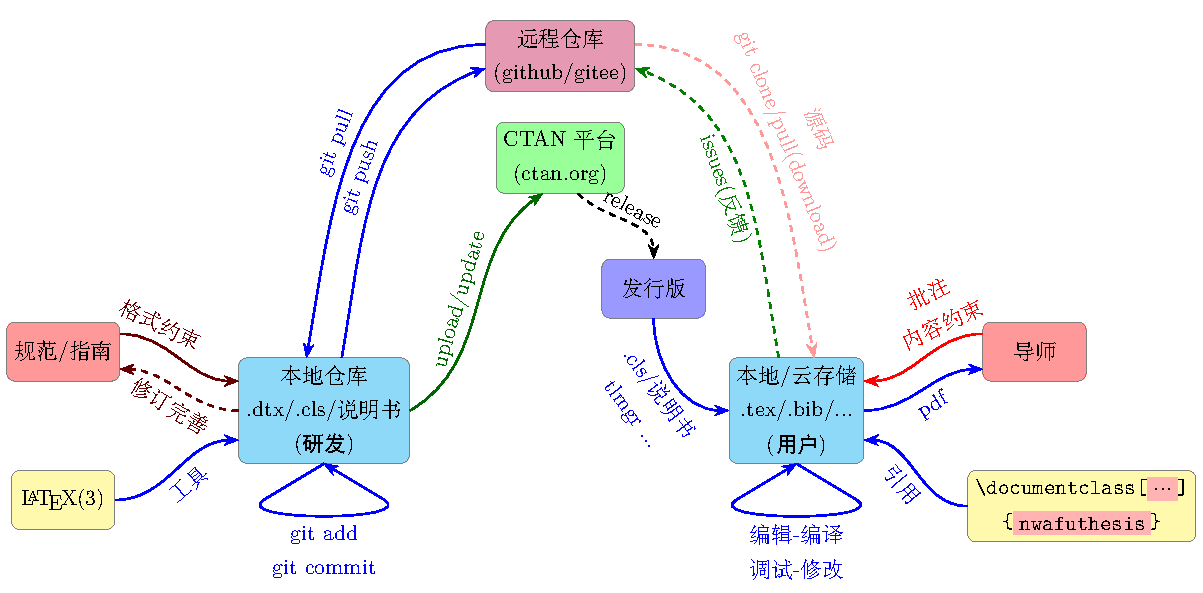
\includegraphics[width=0.85\textwidth]{figs/workflow}
%  \caption{模板工作流}
%  \label{fig:workflow}
%\end{figure}
\begin{enumerate}
	
\item 	数据设计:

GIS系统的数据按照性质的不同可以分为空间数据和属性数据,空间数据指地理空间对象的,属性数据包括地理空间对象的属性以及其他相关联的业务数据等。在了解GIS专题图在采集、存储、分析、研究、图示为一体的数据分析以及GIS专题图对于各种数据格式的定义等知识,GIS专题图的坐标系知识,为(历史、现在、未来)的水系信息,不同区域、时段等粒度的降雨信息,蒸散发信息,地下水信息,地形信息,不同区域粒度的土壤墒情,植被覆盖信息,光照、气温、降水信息,交通信息等为所需设计的雨水资源专题图设计合适的数据格式。
\item 	坐标系设计:

学习GIS专题图坐标系知识,结合系统需求分析以及与雨水资源各种元素因素特性,为雨水资源专题图中各种地形所需的不同的坐标系选择合适的坐标系。如图2所示。
\item	粒度设计

根据水资源不同元素因素的条件(历史、现在、未来)的水系信息,不同区域、时段等粒度的降雨信息,蒸散发信息,地下水信息,地形信息,不同区域粒度的土壤墒情,植被覆盖信息,光照、气温、降水信息等,设计不同时段区域类型等的粒度大小等信息。
\item	应用层设计

本系统的应用层主要是指IE,chrome,firhox等浏览器应用程序。本系统客户端设计采用“瘦客户端”的设计模式,即客户端无需安装任何插件即可进行地图的浏览、查询等操作,降低了对客户端配置的要求,减轻了客户端负担,用户只需普通IE等浏览器即可进行所有操作。本课题以AJAX技术为基础进行GIS专题图的开发,以XML作为与地图服务组件的数据传输协议。大大提升了系统的实用性和可扩展性等能力。
\item	基础底层设计

根据之前的坐标系设计,为不同坐标系下的数据信息设计各自的基础底层,例如地形信息需要基于海拔,地形3D信息的基础底层,而水资源分布只需基于平面的地图便可以表示。
\item 	影响因子设计

不同区域的水资源,如河流、水库、蓄水池、地下水、等水资源信息会受到各
种环境因素如,土壤类型,肥力,墒情,酸碱度,空气温湿度,分数,光照,
经纬度,海拔等因素影响,为了使得水资源信息更加准确,需要设计影响因子
作为水资源分布的参考要素。
\item 	操作图层设计

根据土壤墒情,植被覆盖信息,光照、气温、降水信息,地理信息等影响因子设计操作图层,使用户可以根据不同区域特定情况选择不同影响因子作用下的水资源分布,例如沙型土壤影响因子作用下的地下水的水资源较高,但是对于地表水资源便较少。

\item 	数据获取

采用ArcGIS Server服务,WMS(网络地图服务)、WFS(网络要素服务)等GIS数据服务以及ajax技术实现前后端数据通信,数据的获取。
\item 	数据可视化布局设计

使用OpenLayers和Pvechars库实现对应属性数据的可视化。编写代码实现研究内容中的各种GIS专题图,以及对GIS专题图和数据统计图进行整体组织和布局。
\end{enumerate}
\section{具体设计内容}

研究内容主要为雨水资源管理系统中的雨水资源GIS专题图的设计与实现。


1.	对水资源分布的历史、实时、未来等的信息按照不同的时段、区域、类型等粒度进行统计,并采用统计图(以及列表)的方式进行显示。


2.	水系信息的(历史、现在、未来)GIS专题图制作以及展示。

3.	不同区域、时段等粒度的降雨信息的(历史、现在、未来)GIS专题图制作以及展示。


4.	不同区域、时段、种植作物等粒度的蒸散发信息的(历史、现在、未来)GIS专题图制作以及展示。


5.	地下水信息的(历史、现在、未来)GIS专题图制作以及展示。


6.	地形信息的(历史、现在、未来)GIS专题图制作以及展示。

7.	不同区域粒度的土壤墒情之土壤类型、肥力、墒情、酸碱度等信息的(历史、现在、未来)GIS专题图制作以及展示。

8.	植被覆盖信息的(历史、现在、未来)GIS专题图制作以及展示。

9.	不同区域、时段等粒度的气候之光照、气温、降水等信息的(历史、现在、未来)GIS专题图制作以及展示。

10.	不同区域、时段等粒度的气候之光照、气温、降水等信息的(历史、现在、未来)GIS专题图制作以及展示。

11.	不同区域、时段等粒度的交通信息的GIS专题图制作以及展示。



\section{章节安排}
1.第一章和第二章主要是项目的主要设计内容,研究背景,研究现状以及实现技术等等。

2.从第三章开始为项目的主体介绍,分为三章来介绍项目实现的成果。

3.第三章主要是介绍本项目的需求分析,主要分为:功能需求,性能需求,界面需求,接口需求等。

4.第四章主要介绍雨水资源GIS专题图总体设计,主要为功能设计和数据库设计。

\begin{figure}[H]%关于这些编译器的配置和使用,请参阅相关说明资料。height=0.14\textheight
	\centering
	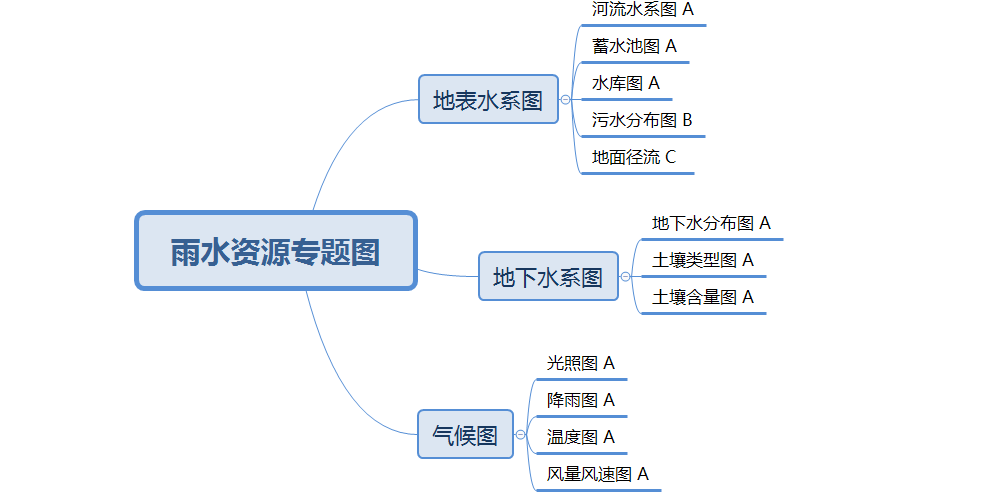
\includegraphics[width=0.60\textwidth]{figs/tree_1.png}
	\caption{雨水资源专题图分类}
	\label{fig:classify_rain}
\end{figure}

5.第五章主要是介绍雨水资源专题图的详细设计与实现以geoserver与openlayers的使用,主要为地表水系图,地下水系图,气候图。地表水系图分为河流水系图、蓄水池图、水库图、污水分布图等,地下水系图主要分为地下水分布图、土壤类型图、土壤含量图等,气候图则主要分为光照图、降雨图、温度图等。如\ref{fig:classify_rain}所示。


%写作过程中的各个文件:
%

%完成部分或所有\verb|*.tex|撰写和修改后,可以在命令行使用 \verb|latexmk -xelatex main|
%进行编译输出\verb|main.pdf|文件,可以根据需要对结果\texttt{pdf}文件进行改名。
%
%也可以使用\texttt{TeXstudio}、\texttt{vscode}等GUI编辑器的进行编辑和编译输出。

%
%
%\note{}由于\nwafuthesis{}需要处理图、表、公式及参考文献等交叉引用,因此,
%往往需要多次编译才能得到正确的结果。为此,必须设置正确的编译方式和编译参数。
%关于多次编译的问题,大家可以浏览耿楠在B站发布的视频
%(\url{https://www.bilibili.com/video/BV1qa4y1v7my?spm_id_from=333.999.0.0})
%进行学习。



%如果论文需要双面打印的话,请务必修改文档类选项,编译双面打印用的 PDF 文件。
%具体地说,在主文件的头部,去除 \texttt{openany, oneside},
%改成 \texttt{twoside}。

%同时,建议注释\cs{nwafuset}命令中的\enquote{style/hyperlink = color},
%以\emph{取消超链接颜色}。

%%% Local Variables:
%%% mode: latex
%%% TeX-master: "../main.tex"
%%% End:
